%*****************************************
\chapter{Der Vergleich mit Sozialen Netzwerken}\label{ch:vergleich}
%*****************************************

Im vorherigen Teil der Arbeit haben wir uns damit beschäftigt, wie soziale Netzwerke so gut und realitätsnah wie möglich konstruiert werden können. Wir haben Analysen durchgeführt und festgestellt, dass die Werte unserer \textbf{Grad-} und \textbf{Nähe-Zentralität} näherungsweise normalverteilt sind. Daher liegt es nahe, weitere sozialen Netzwerke und ihre Analysen zum Vergleich heranzuziehen. Leitfragen sind hierbei, was zu erwarten ist, ob die Ergebnisse den Erwartungen entsprechen oder sogar widersprechen und warum dies der Fall ist. Zusätzlich möchten wir optimalerweise eine Möglichkeit erarbeitet, wie wir unsere Graphen bzw. die Generierung angepasst könnten um vielleicht sogar bessere Graphen zu erhalten, die diesen sozialen Netzwerken noch mehr ähneln. 

\section{Der Datensatz und die Analyse}
Auf der Suche nach vergleichbaren sozialen Netzwerken, beziehungsweise Datensätzen, ist die Suche scheinbar endlos. Auf vielen Webseiten sind große Datensätze für alle Nutzer*innen zugänglich. Meistens als \textbf{CSV} Datei, welche ideal zur Erstellung von Plots, über Sozialen Netzwerken, geeignet sind. In diesem Teil der Arbeit betrachten wir mehrere Datensätze. Natürlich aufgrund der Tatsache, dass sie spannend sind aber auch um mehrere Vergleichswerte zu haben. Starten wir zunächst mit den Daten \cite{GOT} von unserem \textbf{Game of Thrones} Plot \ref{fig:GameOfThrones}. Da wir bereit die Analyse der \textbf{Zentralitäten} und die generelle visuelle Analyse des Graphen durchgeführt haben, reicht uns nun lediglich die Verteilung der Zentralitäten durchzuführen. Die Tabelle mit den Werten der Zentralitätsberechnungen befinden sich erneut in \ref{ch:anhang}. Nachdem wir den Datensatz als \textbf{CSV} Datei in Python eingelesen und zunächst den Graphen folgendermaßen konstruiert:

\FloatBarrier
\begin{figure}[h!]%
  \centering
  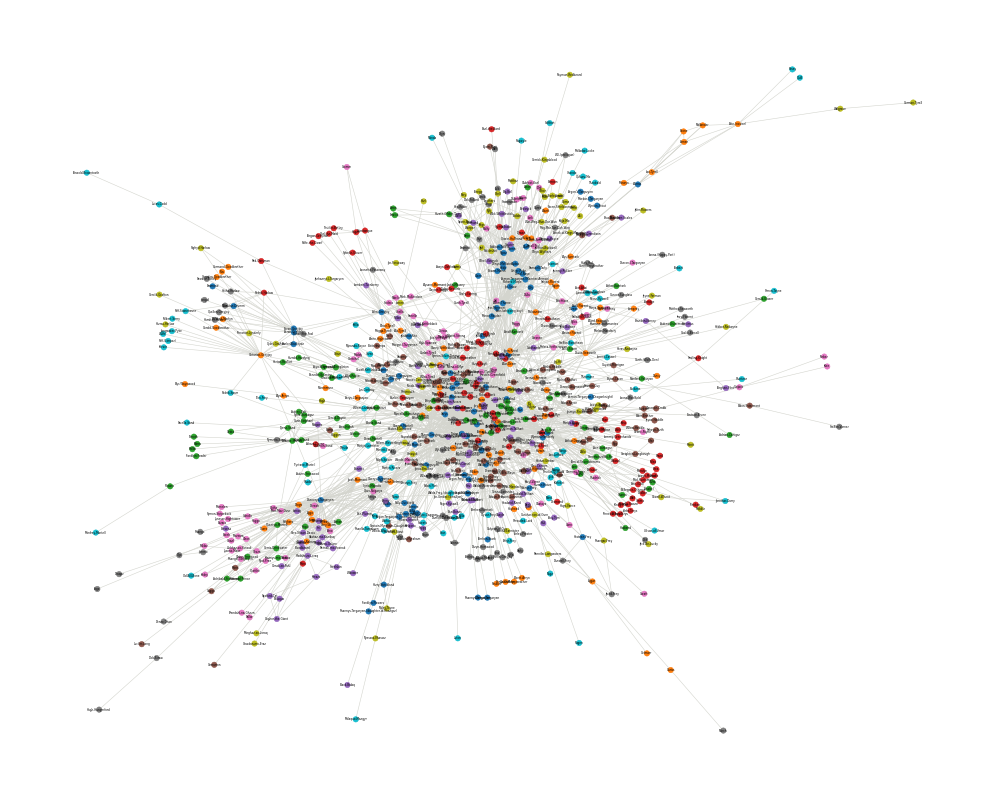
\includegraphics[width=0.5\textwidth]{Graphics/GOTGraph_unweighted.png}
  \caption{Game of Thrones Graph 2.0, \\
  selbst erstellt}
  \label{fig:GOT2.0}
\end{figure}
\FloatBarrier

Dieser Plot ist beabsichtigt klein, da wir ihn lediglich zur Argumentation für die Verteilung der Zentralitäten benötigen und daher die Form des Graphen nur von Bedeutung für uns ist. Zudem ist zu vermerken, dass der eigentliche Datensatz gewichtet ist, und unser Graph daher bereits schon visuell nicht dem Graphen aus \ref{fig:GameOfThrones} ähnelt. Jedoch ist es sinnvoll die Gewichte außen vor zu lassen, da wir in dieser Arbeit ungewichtete Graphen nachbilden. Nachdem wir die Daten des Graphen \ref{fig:GOT2.0} eingelesen, die Zentralitäten berechnet haben und anschließend den Balkengraphen erstellt haben, wurde folgender Plot generiert:

\FloatBarrier
\begin{figure}[h!]%
  \centering
   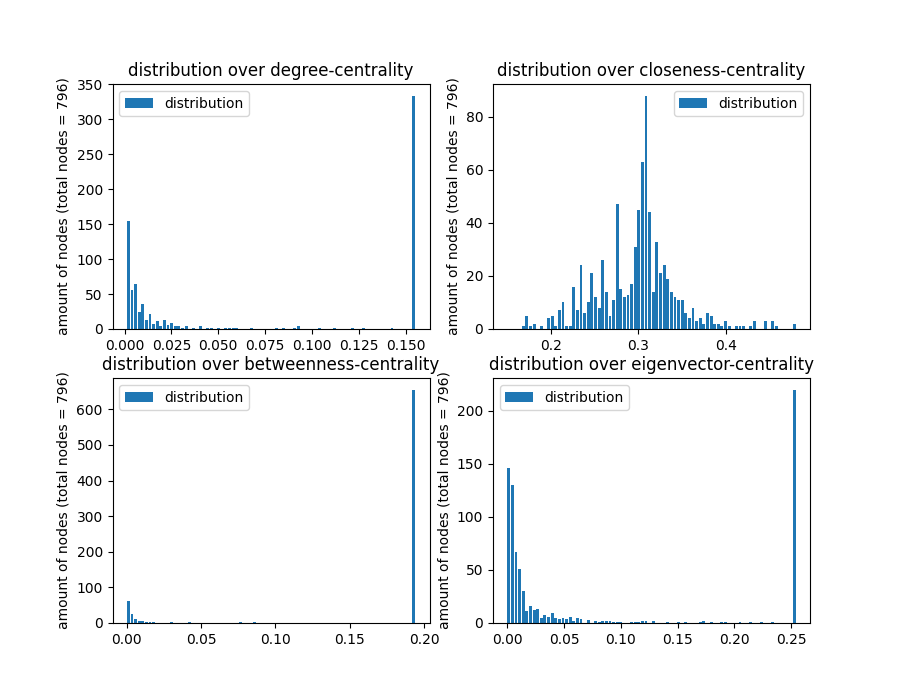
\includegraphics[width=0.8\textwidth]{Graphics/GOTdistribution.png}
  \caption{Game of Thrones Verteilung der Zentralitäten}
  \label{fig:distributionGOT}
\end{figure}
\FloatBarrier
 
 Auf den ersten Blick können wir bereits feststellen, dass wir andere Ergebnisse erwartet haben. Einzig die Verteilung der \textbf{Nähe-Zentralität} ähnelt der erwarteten Normalverteilung. Die \textbf{Betweenness-} und \textbf{Eigenvektor-Zentralität} hingegen ähneln zwar nicht exakt dem, was wir in \ref{fig:distributionALL} herausgefunden haben aber ziehen auf jeden Fall Parallelen. Denn beide haben den Ausschlag im letzten Balken, was wir schon im vorherigen Kapitel damit begründet haben, dass es die Folge davon ist, wenn viele kürzeste Wege stets über die gleichen
Knoten verlaufen, wir also keine Alternativen im Graph haben. Die \textbf{Grad-Zentralität} hingegen darf uns verwundern. Sie ähnelt zum einen stark der Verteilung der \textbf{Eigenvektor-Zentralität} aber keinesfalls der annähernden normalverteilt aus \ref{fig:distributionALL}. Der Ausschlag des letzten Balken ist hingegen schnell erklärt. Wir haben viele Konten, in dem Fall Charaktere, die alle gleich wichtig für den Graphen sind. Diese Konten sind also mit vielen anderen Knoten verbunden, werden daher von vielen anderen Charakteren gekannt oder kennen viele andere Charaktere. Im Allgemeinen sind die Balkendiagramme der \textbf{Zentralitäten} aus \ref{fig:distributionGOT} leider nicht zufriedenstellend. Der Grund, warum die Ergebnisse stark von unseren Erwartungen abweicht ist, dass es sich bei dem Graphen um fiktive Charaktere handelt. Dadurch kann es schnell zu Unstimmigkeiten kommen. Zudem war der Datensatz davor gewichtet, was zu anderen Werten bei der Berechnung der Zentralitäten geführt hätte. Doch wir haben den Datensatz aber ungewichtet betrachtet, um ihn besser mit unseren generierten Graphen zu vergleichen, welche ungewichtet sind. Dies kann auf jeden Fall ein plausibler Grund für Unstimmigkeiten sein. Zudem haben wir die Anzahl der geplotteten Balken stark erhöht und so fallen Unstimmigkeiten auch deutlich stärker auf. Doch wollen wir unsere Theorie, dass Zentralitäten normalverteilterteilt sind, nicht verwerfen und wollen uns ein bis zwei weitere Datensätze anschauen. Als nächstes betrachten wir einen Datensatz, der aus aus "Kreisen" (oder "Freundeslisten") von Facebook besteht. Die Daten wurden anschließend anonymisiert. So können wir mit dem Datensatz also feststellen, ob zwei Nutzer die gleiche politische Zugehörigkeit haben, aber nicht, was ihre individuelle politische Zugehörigkeit bedeutet \cite{FBData}.
Nachdem wir die Daten wieder in eine .CSV Datei umgewandelt und anschließend geplottet haben, konnten wir folgenden Graphen generieren: 


\FloatBarrier
\begin{figure}[h!]%
  \centering
 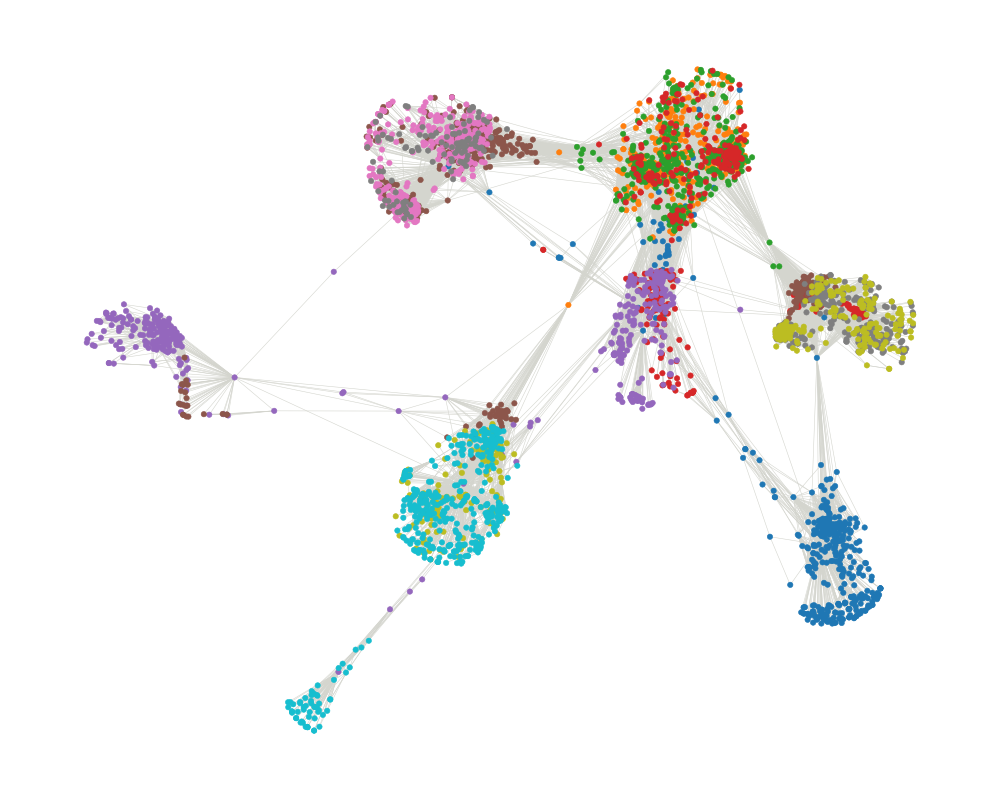
\includegraphics[width=0.7\textwidth]{Graphics/FacebookPoliticalPlot.png}
  \caption{Facebook Graph}
  \label{fig:FacebookGraph}
\end{figure}
\FloatBarrier



Der Graph ähnelt auf den ersten Blick durchaus dem erstellten Plot \ref{fig:SNA}. Sofort fällt aber auf, dass dieser Graph aus deutlich mehr Knoten besteht, zudem weniger Subgraphen aber dennoch im Grunde eine ähnliche Struktur aufweist. Die Berechnungen der Zentralitäten befinden sich auf Github \cite{TZ}. Nun interessiert uns jedoch, wie diese Zentralitäten verteilt sind und ob dieser Graph die erwarteten Verteilungen erfüllen kann. Nachdem wir den Datensatz durch den Code laufen lassen haben, konnten wir folgenden Plot generieren:

\FloatBarrier
\begin{figure}[h!]%
  \centering
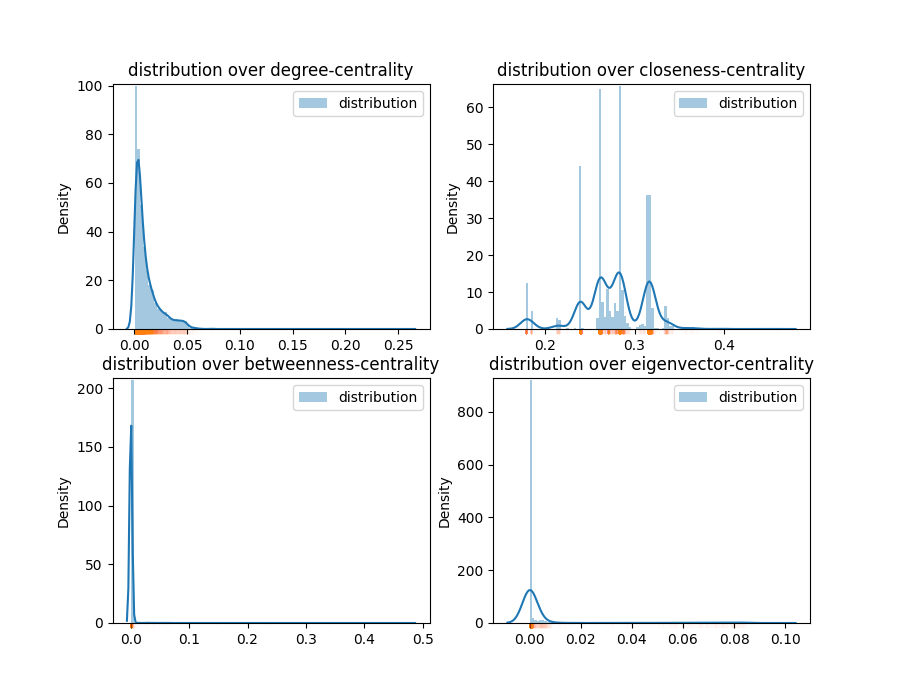
\includegraphics[width=0.8\textwidth]{Graphics/FacebookDistribution.png}
  \caption{Facebook Graph}
  \label{fig:FacebookGraphDistribution}
\end{figure}
\FloatBarrier

Sofort fällt auf, dass wir bei keiner Zentralität eine Normalverteilung sehen. Die \textbf{Grad-Zentralität} fällt uns aber direkt auf, denn es handdelt sich hier um eine Exponentialverteilung. Die anderen Balkendiagramme der \textbf{Betweenness-} und \textbf{Eigenvektor-Zentralität} ähneln jedoch stark den Verteilungen aus \ref{fig:distributionALL}. Was zudem auffällig ist, dass die Diagramm stark an die Verteilungen von \ref{fig:distributionGOT} erinnern. Auch wenn diese Ergebnisse sehr ernüchtern scheinen und vor allem das Balkendiagramm der \textbf{Nähe-Zentralität} sehr eigen. Wir erkennen eine starke Fluktuation der Balken und daher keine schöne Verteilung, die wir aus der Mathematik als Vergleich anbringen könne. Visuell fällt aber  aber visuell auf, dass der Graph \ref{fig:FacebookGraphDistribution} verglichen mit dem Plot des Graphen \ref{ch:SNA} durchaus Parallelen aufweist. Wir sehen deutliche Ansammlungen von Knoten die auch gut als Teilgraphen bezeichnet werden können. Zwischen den Teilgraphen erkenne wir, so wie bei \ref{fig:SNA} einige Kanten, die die Teilgraphen untereinander verbinden. Natürlich weist der obige Graph deutlich mehr Kanten und Knoten auf. Unsere Graphen haben im Schnitt um die \textbf{950} Knoten und \textbf{8700} Kanten, daher also circa neun mal so viele Kanten wie Knoten. Auch haben wir im Schnitt um die \textbf{10100} Cliquen, welche maximal acht Knoten groß sind. Bei dem Facebook Graphen \ref{fig:FacebookGraph} hingegen sprechen wir von \textbf{4093} Knoten und \textbf{88234} Kanten. Das heißt circa einundzwanzig mal so viele Kanten wie Knoten. Doch als wir unsere Kanten und Knoten im Code erhöht haben, um ebenfalls die selbe Relation zu erhalten, waren alle vier untersuchten Zentralitäten annähern Normalverteilt. Was zum einen daran liegt, dass wir letztendlich Graphen wie \ref{fig:GOT2.0} erhalten haben, die noch viel dichter besetzt waren. Wir können festhalten, dass sich die \textbf{Betweenness-} und \textbf{Eigenvektor-Zentralität} bei allen unsersuchten Datensätzen stark zu unseren Verteilungen des künstlich generierten sozialen Netzwerk ähneln. Auch die die \textbf{Nähe-Zentralität} weist stets ähnliche Verteilungen auf, was die Korrektheit des Graphen \ref{fig:SNA} bestätigt. Doch wundert uns nach wie vor die Verteilung der \textbf{Gradzentralität} weshalb wir noch einen letzten Datensatz untersuchen wollen. 


\todo{noch mehr zu Cliquen und Brücken}
\todo{besseren Datensatz}
\todo{Argumentation wie bei mein Graph dann Verteilung wurde als ich ihn noch angepasst hatte}
\todo{Argumentation warum Differenzen}
\todo{Ausblick und Fazit}

